\documentclass[letterpaper,12pt,twoside=false,DIV=11]{scrartcl}

%----------------------CONFIG---------------------------
%math packages
\usepackage{amsmath,amssymb,amsthm,units,unitsdef}

%bibliography style and citation style, bibstyles to use: plainnat, abbrvnat, unsrtnat, named, chicago
%otherwise numerical citationstyle will be used
%\usepackage[authoryear,round]{natbib}

\usepackage{longtable,tabularx,tabulary,multirow,lscape}
\usepackage[font={sl},format=plain,labelfont=bf]{caption}

% colors
\usepackage{color,colortbl}
\usepackage[dvipsnames]{xcolor}
\definecolor{darkblue}{HTML}{00354C}

\usepackage{booktabs}
%\usepackage{showkeys} % shows the labels above the references for

%easier development
\usepackage{ifpdf}

\ifpdf
    \usepackage[pdftex]{graphicx}
    \usepackage[]{pdfpages} %for including full pdf pages
    \usepackage[pdftex,
        bookmarks,
        bookmarksopen=true,
        bookmarksnumbered=true,
        pdfauthor={Reto Trappitsch},
        pdftitle={On the origin of elements in the Milky Way - Homework},
        colorlinks,
        linkcolor=darkblue,
        citecolor=darkblue,
        filecolor=black,
        urlcolor=darkblue,
        anchorcolor=black,
        menucolor=black,
        breaklinks=true,
        pageanchor=true, %for jumping to a page
        plainpages=false,
        pdfpagelabels=true]{hyperref}
    \pdfcompresslevel=9
    \pdfoutput=1
    \DeclareGraphicsExtensions{.pdf,.png,.jpg,.jpeg}
\else
    \usepackage{graphicx}
\fi
\usepackage{rotating} % rotate figures
\usepackage{subcaption}
\usepackage{wrapfig}


\usepackage{fancyhdr}
\pagestyle{fancy}
%\addtolength{\headwidth}{\marginparsep} %these change header-rule width
%\addtolength{\headwidth}{\marginparwidth}
\lhead{}
\chead{\small\scshape On the Origin of Elements in the Milky Way} 
\rhead{} 
\lfoot{} 
\cfoot{\thepage} 
\rfoot{} 
\renewcommand{\headrulewidth}{.3pt} 
\renewcommand{\footrulewidth}{.3pt}

% Redefine author as topic
\newcommand{\topic}{\author}

%
%Redefining sections as problems
%
\makeatletter
\newenvironment{problem}{\@startsection
    {section}
    {1}
    {-.2em}
    {-3.5ex plus -1ex minus -.2ex}
    {2.3ex plus .2ex}
    {
        \pagebreak[3] % forces pagebreak when space is small; use \eject for better results
        \noindent\sffamily\bfseries Problem
    }
}
{
    %\vspace{1ex}\begin{center} \rule{0.3\linewidth}{.3pt}\end{center}}
    \begin{center}\large\bfseries\ldots\ldots\ldots\end{center}
}
\makeatother

% set enumerate to use letters
\renewcommand{\theenumi}{\alph{enumi}}

% newcommands
%============
% my short cuts
\providecommand{\e}[1]{\ensuremath{\times 10^{#1}}}
\providecommand{\ex}[1]{\ensuremath{^{#1}}}
\providecommand{\dex}[1]{\ensuremath{\delta^{#1}}}
\newcommand{\nean}{$^{22}$Ne($\alpha$,n)$^{25}$Mg}

% textnormal
\newcommand{\tn}{\textnormal}
% textregistered
\newcommand{\tr}{$^\tn{\textregistered}$}


%-------------------DOCUMENT---------------------------

\begin{document}


\title{Homework \#4 -- Solution}
\topic{Massive stars, \emph{s}-process nucleosynthesis}
\date{}

\maketitle
\thispagestyle{fancy}

\begin{problem}{Isotope Abundances in the Iron Peak (20\%)} \label{prob1}

Most of the iron-peak elements are produced by combining $\alpha$ nuclei. Combining 14 on these results in \ex{56}Ni, which decays via $\beta^{+}$ decay to \ex{56}Co and then \ex{56}Fe. Iron-58 and \ex{62}Ni, however, are not on the $\alpha$ chain. Therefore, they are produced in lower abundances compared to \ex{56}Fe, even though they have higher binding energies per nucleon.

\end{problem}

\begin{problem}{Supernova Explosion Energy (20\%)}

Making \ex{56}Fe from hydrogen would release for every \ex{56}Fe made a total of 8.7903\,MeV per nucleon. With 56 nucleons, this means that a total of 492.2568\,MeV would be released. This is equal to a release of $7.88\times10^{-11}$\,J per creation of \ex{56}Fe. The energy release in a supernova is 100\,foe, which is equal to $10^{46}$\,J. This means that a total of $1.26\times10^{56}$ \ex{56}Fe could be produced. The molecular mass of \ex{56}Fe is about 56\,g\,mol$^{-1}$. Thus, around $1.2\times10^{31}$\,kg of \ex{56}Fe could be produced with 100\,foe of energy, which is equal to around $6\,M_\odot$.

\end{problem}

\begin{problem}{Local Approximation (20\%)}
\begin{center}
    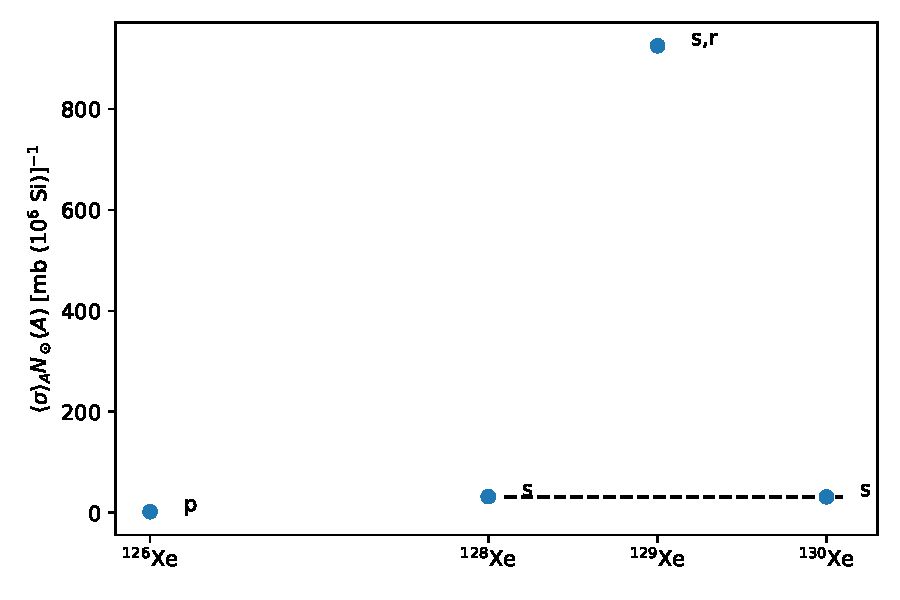
\includegraphics[width=0.75\textwidth]{local_approx_xe}
\end{center}
\begin{enumerate}
    \item These two isotopes are \emph{s}-only isotopes and are shielded from the \textit{r}-process. These isotopes are also far from neutron magic numbers and thus adhere to the local approximation.
    \item There is no stable isobar that shields \ex{129}Xe from the \textit{r}-process. It has therefore a mixed production of \textit{s}- and \textit{r}-process and does not adhere to the local approximation. Note that the $r$-process can be estimated by calculating how much of this nuclide is produced by the $s$-process, since the $s$-component would adhere to the local approximation.
    \item Finally, \ex{126}Te is shielded from the $r$-process, however, cannot be produced by the $s$-process. It is thus a proton-rich nuclei with a different origin, and therefore does not adhere to the local approximation.
\end{enumerate}
\end{problem}

\begin{problem}{Exploring a Star (40\%)}

\begin{enumerate}
    \item The black curve in Figure 111 shows the C/O ratio inside the star. After each third dredge-up event, this ratio in the envelope increases and the star becomes more carbon rich.
    \item Figure 107 shows that the star looses most of its mass in the last thermal pulse. Starting off with $2\,M_\odot$, the star looses around $0.5\,M_\odot$ in the last thermal pulse and a total of around $0.5\,M_\odot$ in all preceding pulses. It is therefore left, after strong stellar winds, with about half the mass it started with.
    \item Figure 124 shows produts of the $s$-process in the intershell. A clear $s$-process isotope, and the one with the widest distribution, is \ex{86}Sr. Let us use this isotope to constrain the maximum extension of the \ex{13}C pocket. In width the production of \ex{86}Sr goes from $0.603153\,M_\odot$ to around $0.603171\,M_\odot$. This means that the \ex{13}C pocket is around $1.8\times10^{-5}\,M_\odot$ wide. This is fairly small compared to the size of the whole star.
    \item Clearly, the most abundant isotope is \ex{56}Fe, the seed of the $s$-process. While the strong $s$-process, which takes place in TP-AGB stars, makes all $s$-isotopes starting at strontium, the seed is barely destroyed. There is simply far too much \ex{56}Fe in the star to have a significant effect. For $A>80$ the two most abundant isotopes are \ex{88}Sr and \ex{138}Ba.
    \item Both, \ex{88}Sr and \ex{138}Ba are neutron magic. Thus, their MACS are very small and pile-up of these isotopes will take place during the $s$-process. This explains why they are the most abundant isotopes with $A>80$ in the $s$-process
\end{enumerate}

\end{problem}

\end{document}
